\chapter{Gates und Eventgrenzen}
\label{ch:untersuchung}
Nun haben wir also Neuronale Netz mit LSTM Speicherzellen auf verschiedene Fälle des Bouncing Ball Szenarios trainiert. Wenn man dabei die internen Aktivierungen der Gates über die Zeit betrachtet und vergleicht mit dem Verlauf der Ereignisse der trainierten Aktion, findet man Zusammenhänge. In diesem Kapitel werden wie erst Beispiele für solche Zusammenhänge betrachten, dann schauen wie man diese automatisiert finden kann. Zum Schluss schauen wir noch, wie wir mit Hilfe von Backpropagation through time Vorhersagen über Events anhand der Gate-Aktivierungen treffen können und wir dieselbe Technik nutzen können um die Eventbeziehungen zu klassifizieren.
\section{Gate-Aktivierungen}
Die Möglichkeiten wie sich eine LSTM über die Zeit verhalten kann sind zahlreich, noch zahlreicher die Möglichkeiten wie mehrere von ihnen miteinander interagieren. 


\begin{figure}
	\centering
	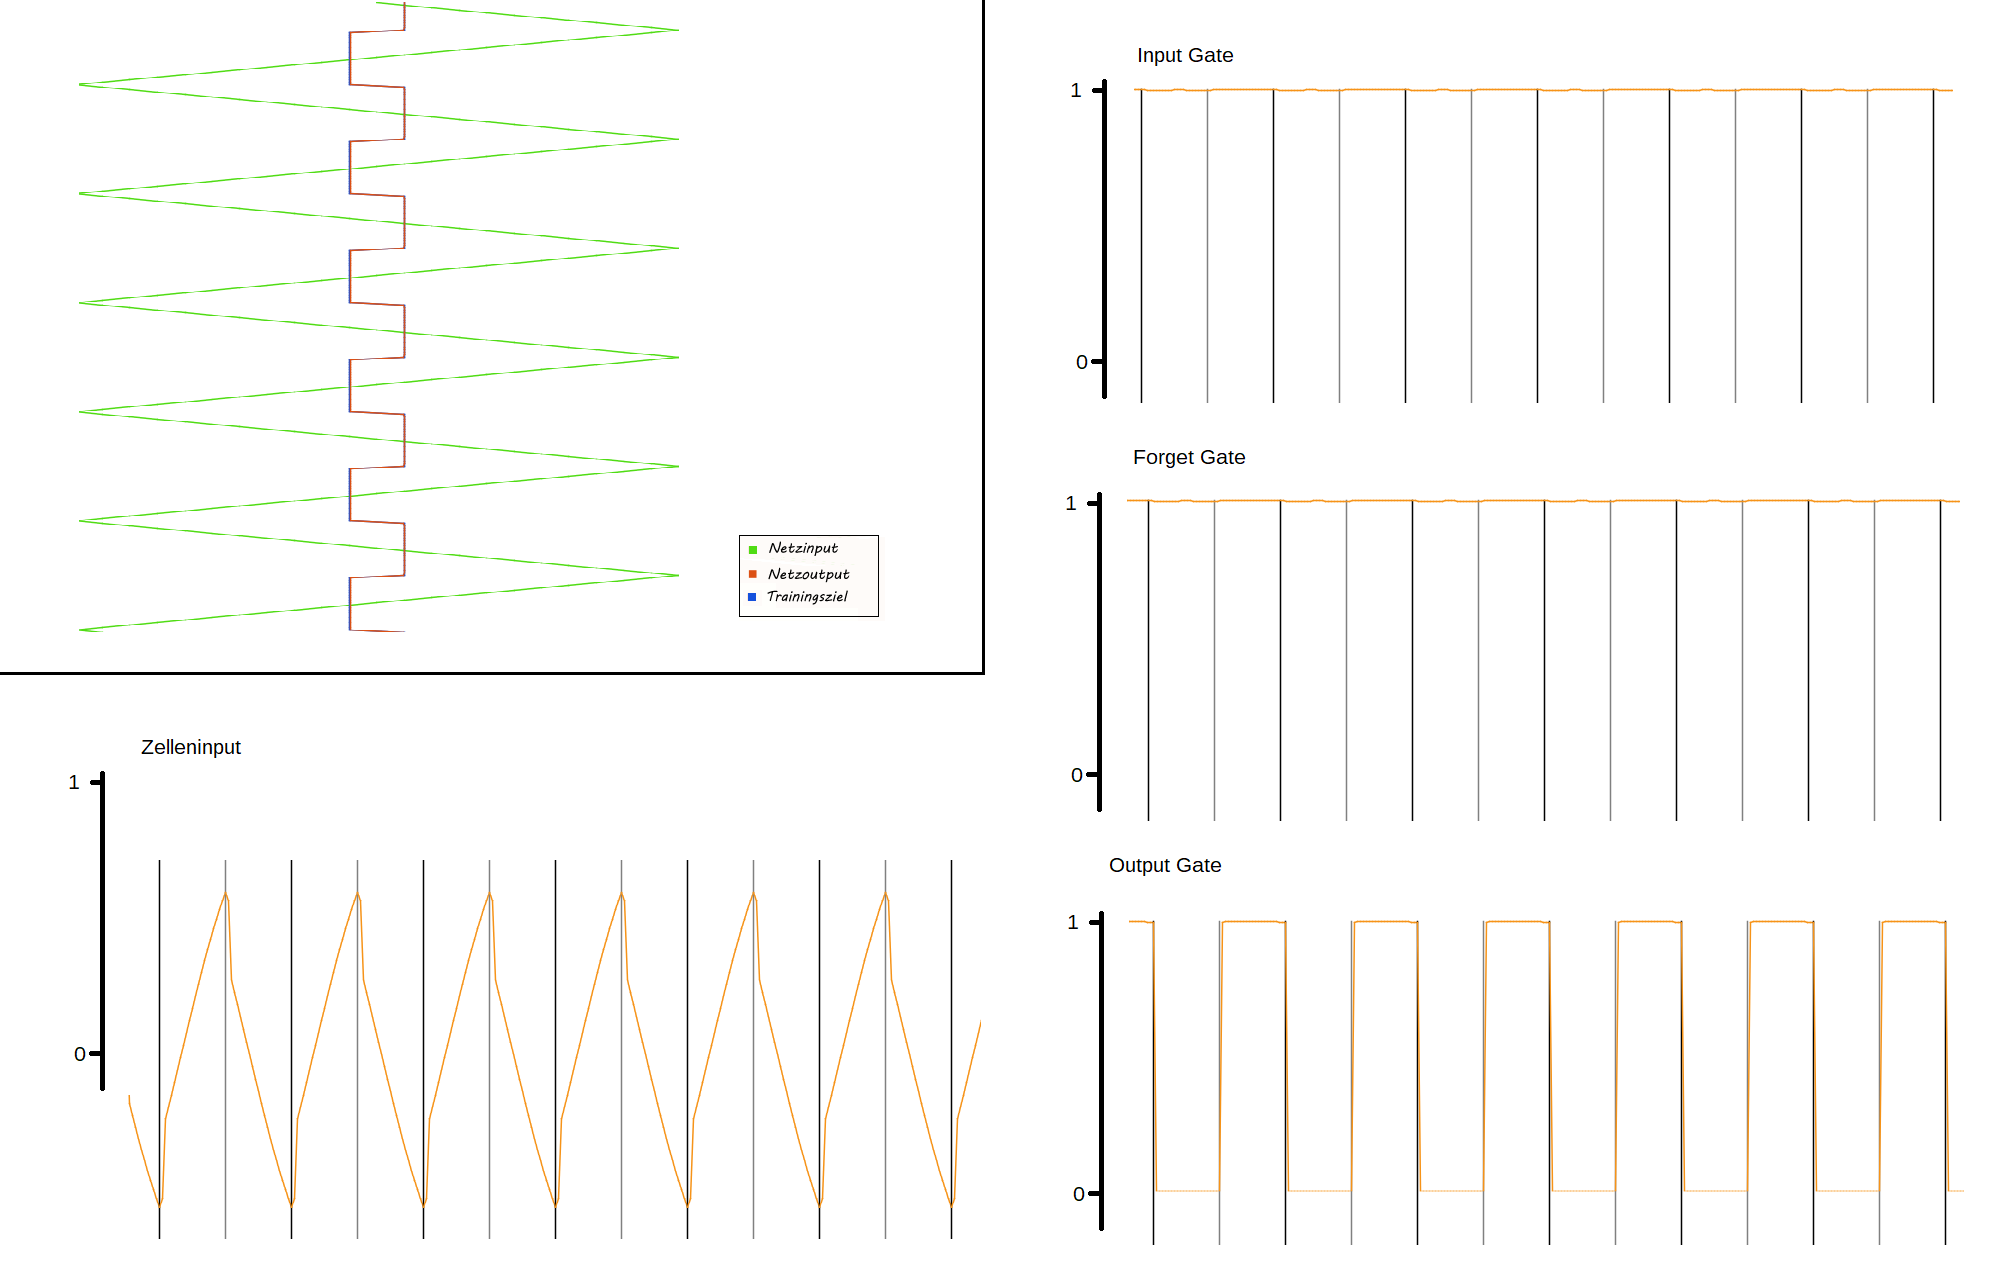
\includegraphics[width=0.9\textwidth, height=400px]{pics/act1.png}	
	\caption{Der 1D Fall mit Ballposition als Netzinput und nächste Geschwindigkeit als Trainingsziel, gelernt von einem 1-1-1 Netz.  }
	\label{img:act1}
\end{figure}


\cite{bib:graves}

\section{Automatisierte Klassifizierung}




\section{Analyse mit BPTT}

periodisch: sieht man immer, das nicht das problem, sogar klar. overfitting

Verhalten an der Eventgrenze:

runde annäherung nicht erwünscht, aber wird es immer sein nur eben immer unrunder. im besten fall, dauert die eventgrenze immernoch über 4 zeitschritte an(1D-Fall), was durch Diskretisierung abgehackt aussieht, aber doch eine kurve ist bei kontinuierlich




RNN Annäherung vs echte nichtlinearität

anders als angenommen: zufall war garnicht wichtig. Alles was bestätigt wurde, 2 1D Fälle überlagert

dieser fall den man bekommen hätte mit feedback und zufällig und perfekt trainiert, vllt sogar viel langweiliger, da event tatsächlich nur von position des Balles abhängt, nur ein einzelnes Gewicht, wenn 1 erreicht ausgelöst ohne interaktion. 


mit backpropagation im 1D fall, sieht man: Lstm zelle forgetgate ist auf 1. wir bewegen uns nach links. wenn man gradient +1 wählt, kommt dann auf selbe zelle negativer gradient zurück? also um wieder nach links zu gehen muss man erstmal nach rechts gehen. 

Wunschergebniss, falls man es nicht sieht beschriebe es un erzähle warum man es nicht sieht: 
Hat ein Netz ein Event gut gelernt, merkt man das auch anhand der Zellen die eventeinteilung klappt besser.
Dierekter zusammenhang: lstm netz gut trainiert, mlp zur est gibt gute ergebnisse.

Wunschergebniss
Unterschiede zwischen random und nicht random
Bei random funktioniert est viel besser,  da  durch unterschiedliche geschwindigkeiten die eventkanten besser gelernt werden müssen, bzw bei nicht random werden periodische funktionen gelernt die die event segmentation behindern.

Vergleiche: Testfälle Random 1 und Random 2 Richtungen. Inwiefern weisen die LSTM zellen hinweise auf eventsegmentation? 

Vergleiche: 2D mit 6-8 und 16 zellen gelernt.
Und mit 4? Was ist die kritische Zahl?

Erstelle eine Ansicht, die anzeigt welche Zellen und Werte genutzt wurden.

Stelle 2 Hypothesen auf was den in den Gates untersucht wird, ist es ob ich mich grad nach oben rechts bewege oder das oben und links die letzten Events stattgefunden haben.

Teste 2 verschiedene mlp formen: 4 outputs für wahrscheinlich des nächsten events,
oder 2 outputs für wahrscheinlich das jeweils konträre die nächsten sind.


Vorzeigefall: Rekurenz grundding: Gleicher Input kann abhängig von vorigen stats unterschiedlichen outputs leifern, man befindet sich dank lstm auch in unterschiedlichen gatepositionen.
Zeige ball der in 0,0 sitz der nach unten rechts un nach oben links fliegt und die aktivierungen

Feedback sollte integriert werden, um die eventtransition mehr zu werden. Darlegen warum event sauberer is wenn feedback benutzt ist. Vllt hätte das auch zu klareren events geführt. Für klarrerer events wurde auch neues random entwickeld bei dem die kante bei jedem step sauber getroffen wird.

Kann MLP abschätzen wie Nahe das Event ist?
Verschiedene Thresholds, Event in 2 Steps, 5 Steps, 10 Steps, Alarm geben wenn Kollision bevorsteht.

Erklären wie die Trainingsdaten für das mlp aussehen

Vergleiche mlp das next und last event sagt
Vorhersage: last event exakt deutlich, next event unklarer das ob oben oder rechts als nächstes getroffen wird vom vall abhängt wenn man von links unten kommt-

Wichtig:
Vergleiche im LSTM die bedeutung der einzelnen Gates auf EST. Zentral
